\chapter{Introduction}
\section{Dimensional Analysis and SI units}
The \textbf{SI}\index{SI system of units} system of units is the standard used by many scientists throughout the world.  There are seven \textit{fundamental} or \textit{base} quantities from which all other measurements are derived.  These quantities are listed below:
 \index{Units, Fundamental}

\begin{center}

	
\begin{table}[ht]\caption{\textbf{SI Units}}% title of Table 
	\centering % used for centering table	
	\begin{tabular}{|c|c|c|}
		\hline \hline
		\textbf{Quantity} & \textbf{Unit} & \textbf{Unit Symbol}\\
		\hline
		time & second & s \\
		\hline
		length & meter & m \\
		\hline
		mass & kilogram & kg \\
		\hline
		electrical current & Ampere & A \\
		\hline
		temperature & Kelvin & K \\
		\hline
		amount of substance & mole & mol \\
		\hline
		luminous intensity & candela & cd \\
		\hline		
	\end{tabular}
	\label{table:nonlin}% is used to refer this table in the text
\end{table}
\end{center}

	Of these quantities, mass, time and length are quite common.  Thus, this system is sometimes called the MKS (meter, kilogram, second) system. In order to use any equations, all measurements must have correct units.  For example, if a time is expressed in hours, it must first be converted into seconds before any calculations can be attempted.  
	
	Dimensional analysis \index{Dimensional Analysis} is the process in which the units associated with quantities create \textit{derived units}. \index{Units, Derived} For instance, when a distance is divided by a time, the units will be $ \frac{m}{s}$ (read \textit{meters per second}).  	
	
	Dimensional analysis is an important part of solving physics problems.  Often, correct dimensional analysis can help you determine if a problem has been solved correctly.  One should not even attempt to calculate an answer to a problem until the correct units have been verified. 



		


\section{Vectors and Scalars}
In the study of physics, there are two types of quantities that we will deal with on a regular basis: \textit{scalars} and \textit{vectors}.  

A \textbf{scalar} is a quantity that you are already most likely very familiar with, as it is just a number; scalars have only a \textit{magnitude} (a number that represents how big or strong it is), and can sometimes include units.  Examples of scalars might be the number of people in a room, the mass of a car, or your age in years.  

\textbf{Vectors} are different from scalars because in addition to a magnitude, they contain a direction as well.  Examples of vectors might include 50 feet to the north, 5 m/s at a 33$^\circ$ angle, or 200 miles straight up.  
There are many ways of expressing vectors.  Symbollically, they are often written with an arrow over them.  For example, in the equation \color{blue} $\vec{F} = m \vec{a}$ \color{black}  both force and acceleration are vectors – meaning that both force and acceleration have a direction.  Sometimes vectors will be expressed in \textbf{bold} typeface.   Hence, the expression \\ \color{blue} \textbf{F} = m \textbf{a}  \color{black} is equivalent to the expression shown above.

The direction for vectors in 1 dimension is easy – all you need is a positive or a negative.  Usually, 1-dimensional motion takes place along the x-axis (left and right), but sometimes it will take place in the y- (forward and backward) and z- (up and down) dimensions.  For the purposes of this book, positive is to the right and up unless otherwise stated. 
In two dimensions, a vector requires two pieces of information.  One way of expressing a vector is in polar form.  Polar form in two dimensions includes a magnitude of the vector and an angle, usually measured from the x-axis.  There are several ways for writing this.  4 cm @ 15$^\circ$, \\ 4 cm $\angle 15^\circ$ and 4 cm at 15$^\circ$ North of East all represent the following displacement vector:
	\begin{center}
		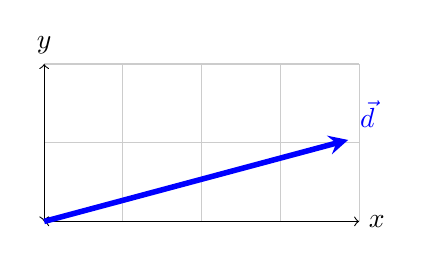
\begin{tikzpicture}
		\draw[thin,gray!40] (0,0) grid (4,2);
		\draw[<->] (0,0)--(4,0) node[right]{$x$};
		\draw[<->] (0,0)--(0,2) node[above]{$y$};
		\draw[line width=2pt,blue,-stealth](0,0)--(3.86,1.035) node[anchor=south west]{$\vec{d}$};
	
		\end{tikzpicture}
	
	
	
	\end{center}

	
	Unit vectors are vectors that have a length of one unit and are oriented along one axis.  The unit vector for the x-direction is written as $\hat{i}$ (pronounced i-hat).  $\hat{i}$ is a 1-unit long vector that is always parallel to the x-axis, and points in the direction of increasing x values.  Likewise, the y-direction and z-direction unit vectors are written as $\hat{j}$ and $\hat{k}$ respectively.  
	
	
	Because the surface of a paper is effectively 2-dimensional, it is very hard to draw lines that are oriented directly into or out of your paper. For this purpose, physicists have agreed to the following convention: vectors that point directly into your paper are notated by $\bigotimes$ .  Vectors that point directly out of your paper are shown by the symbol $\bigodot$.  
	
	Sometimes, vectors may be expressed in Cartesian coordinates.  This vector could either be expressed as an ordered pair (or triple) with square brackets, such as [3, 4, 5] cm, or as a linear combination of the unit vectors shown above, such as $5\hat{i} + 12 \hat{j} + 3 \hat{k}$  In each case, the distances in each direction are given by the numbers shown.
	
	When converting between polar and cartesian forms for two dimensional vectors, a little trigonometry shows: 
	\color{blue}
	\begin{multicols}{2}
		\begin{center}
			\begin{equation}
			x = r \cos(\theta)
			\end{equation}
			
			\begin{equation}
			y = r \sin(\theta)
			\end{equation}

			\begin{equation}
			r = \sqrt{x^2+y^2}			
			\end{equation}

			\begin{equation}
			\theta=\tan^{-1}(\frac{y}{x})
			\end{equation}		
		\end{center}
	\end{multicols}
	\color{black}
	In three dimensions, polar form comes in two types – Cylindrical and Spherical.  In cylindrical coordinates, expressed as [r, $\theta$, z],  the above conversions are used, and the z-coordinate remains unchanged from Cartesian form.  We will study spherical coordinates more in \color{red} INSERT REFERNCE HERE! \color{black}
	
	
	
	
	
\section{Vector Mathematics}
	\subsection{Vector Addition}
	\subsection{The Dot Product}
	\subsection{The Cross Product}
	
